
As shown in \cref{fig:diagram_Connectivity-Activity}, our idea for connection inference rests on the causal `presynaptic spike' → `postsynaptic voltage bump' link. I.e. we want to know for which neuron pairs a spike in one is reliably followed by such a bump in the other. The problem is that these bumps (the postsynaptic potentials or PSPs) are minute, and are easily drowned out by (1) other PSPs, (2) postsynaptic spikes, and (3) voltage imaging noise.

So, as is often done in neuroscience, we take the \emph{average} over many instantiations, so as to hopefully find a signal in the noise. Specifically, we take spike-triggered averages, or \textbf{STA}s, of neurons' voltage traces. If there is a connection from neuron `1' to neuron `2', then an STA of neuron 2's voltage imaging signal, based on neuron 1's spikes, would hopefully show the PSP.

To use this idea for an actual connection test, we look specifically at the height of an STA, and compare it to a distribution of STA heights that we'd expect were the two neurons not connected. This is illustrated in \cref{fig:STA-height-suffle}.


\begin{figure}
    \vspace*{2em}
    \hspace*{-1em}
    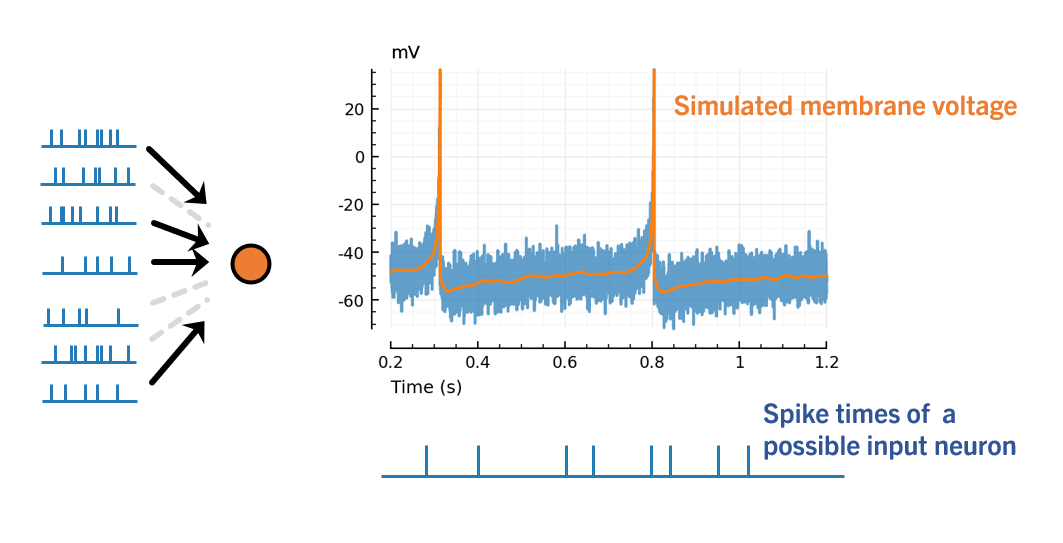
\includegraphics[w=1.2]{diagram_Nto1.png}
    \vspace*{-1.4em}
    \captionn
        {The `N-to-1' problem}
        {\Left: A neuron $N$ (orange circle), and the spike trains of other neurons in the network (blue). Some of these other neurons impinge directly on $N$ (black arrows), while others are not (directly) connected (dashed gray lines). Given only neuron $N$'s voltage signal and the other neurons' spiketrains, we want to detect the direct inputs, while rejecting the not-directly-connected spiketrains.\newline
        \Right: The simulated membrane voltage of the impinged-upon neuron (orange), and the same signal with Gaussian noise added, to simulate a voltage imaging signal (blue). Underneath the plot, one of the possible input spiketrains, time-aligned to the voltage signal.
        This alignment is used later to extract spike-triggered windows from the voltage signal.}
    \label{fig:diagram_Nto1}
\end{figure}

\begin{figure}
    \hspace{-5em}
    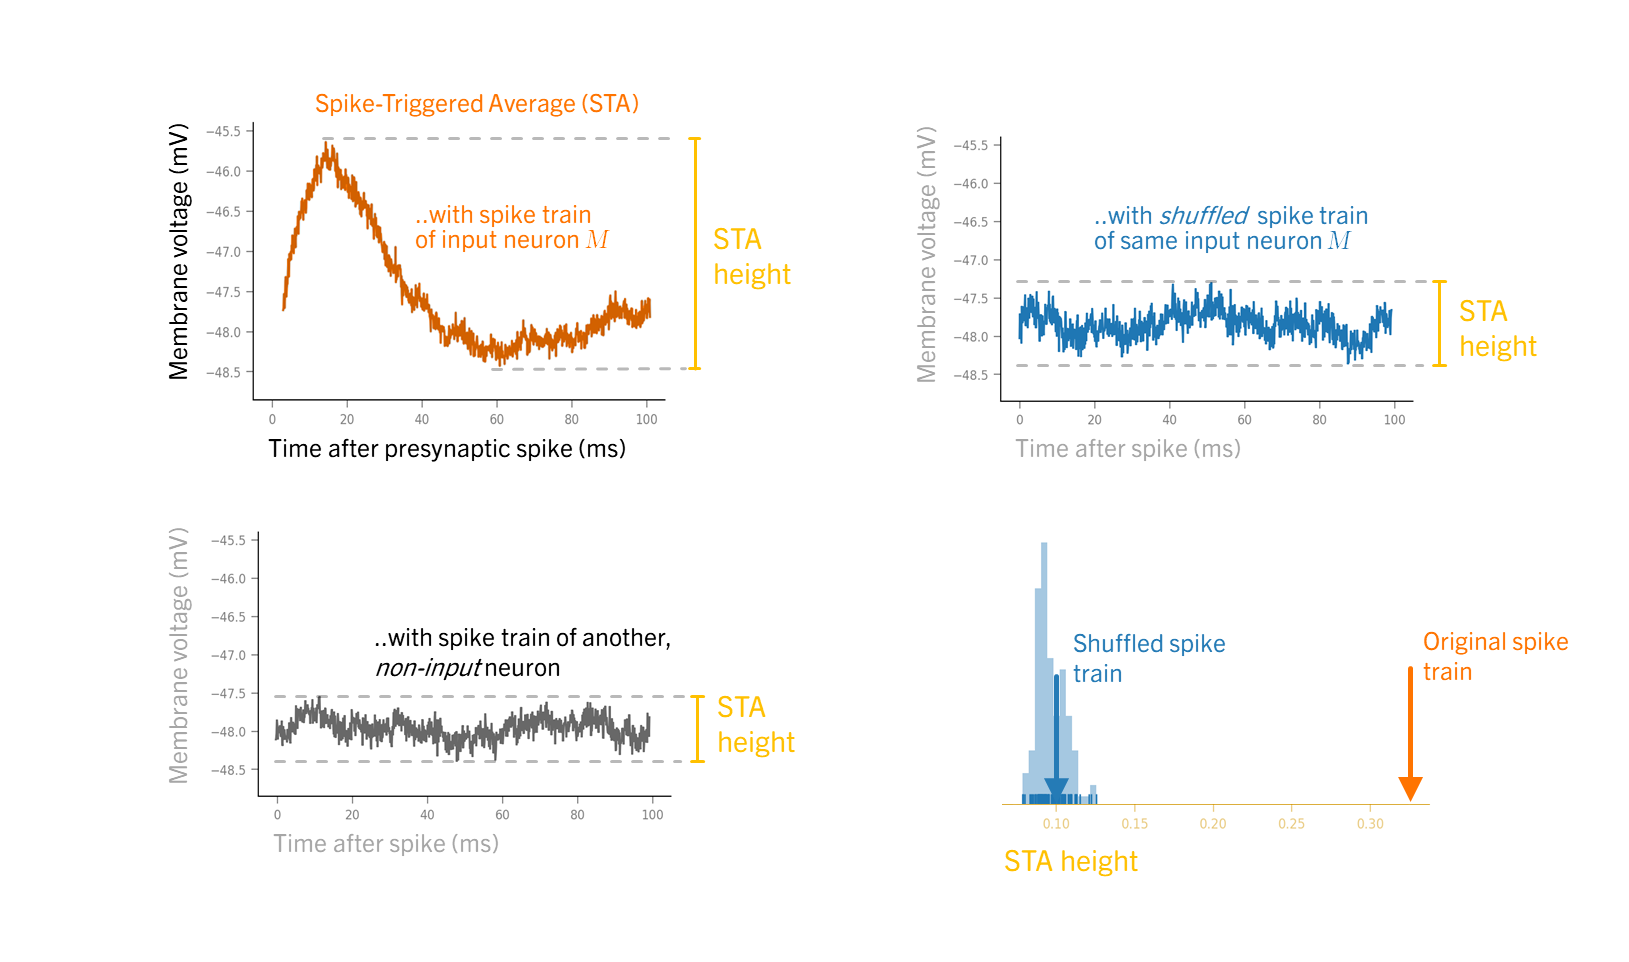
\includegraphics[w=1.7]{diagram_STA_test.png}
    \captionn
        {A simple connection test: STA height with shuffle control}
        {The spikes of a possible input neuron are aligned to the voltage trace of the neuron of interest $N$, as in \cref{fig:diagram_Nto1}. For every such spike, a 100-ms long window is cut out of the voltage of $N$. The average of all these windows is called the spike-triggered average (STA).\newline
        \Left: Two example STAs of neuron $N$'s membrane voltage: one for an actually connected input neuron, $M$ (top, orange); and one for a non-input neuron (below, gray).
        Given an STA signal $x$, we will use its height $h = \max(x) - \min(x)$ (also known as `peak-to-peak' or `ptp') to test whether two neurons are connected. \newline
        \Right: An STA of $N$'s membrane voltage using a shuffled version of $M$'s spike times (which is made by randomly permuting the inter-spike-intervals of $M$). This `shuffled STA height' provides a control for the STA height connection test statistic: "what do we expect the STA height to be if there is \emph{no} connection $M$→$N$".
        By calculating different such shuffles, we obtain a null-distribution for the STA height test statistic. And by comparing the real STA height to this distribution, we can calculate a $p$-value. Here, the real STA is larger than all shuffle controls, of which there are 100. So $p < 0.01$, and at α = 0.05, we conclude there is indeed a connection $M$→$N$.}
    \label{fig:STA-height-suffle}
\end{figure}

\begin{figure}
    \hspace*{-3em}
    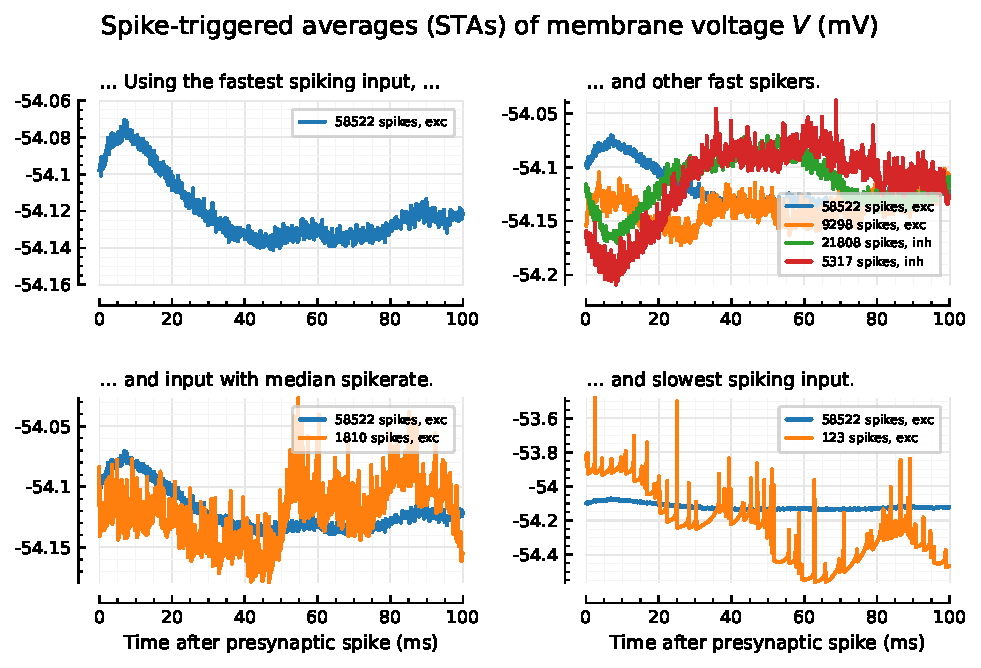
\includegraphics{example_STAs}
    \vspace*{1em}
    \captionn
        {Example STAs in the 10' simulation with 6500 inputs}
        {
        Note that every panel has a different y-axis (voltage) scale. The STA of the most active input is repeated in every panel (in \mpl{blue}), to allow a visual scale comparison nonetheless.\\
        The inset legends indicate with how many presynaptic spikes the STA was calculated, and whether the input was an excitatory or inhibitory one.\\
        The top right panel shows STAs of the 1\ts{st} and 100\ts{th} fastest spiking inputs, both within the excitatory inputs (\mpl{blue} shades), and within the inhibitory inputs (\mpl{orange} shades).\\
        Source: \nburl{2023-09-13__Clippin_and_Ceilin}.
        }
\end{figure}



\section{Ceiling and clipping}

\begin{figure}
    \begin{sidecaption}
        {}
        [fig:ceil_n_clip_sigs]
        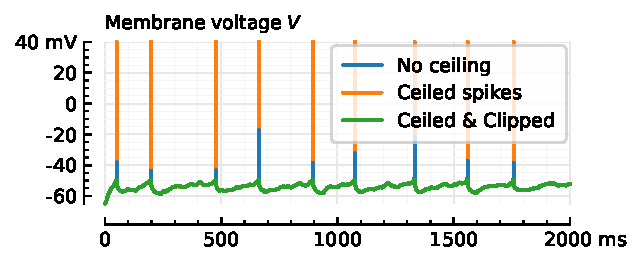
\includegraphics[w=1]{ceil_n_clip_sigs}
    \end{sidecaption}
\end{figure}

\begin{figure}
    \begin{sidecaption}
        {}
        [fig:ceil_n_clip_STAs]
        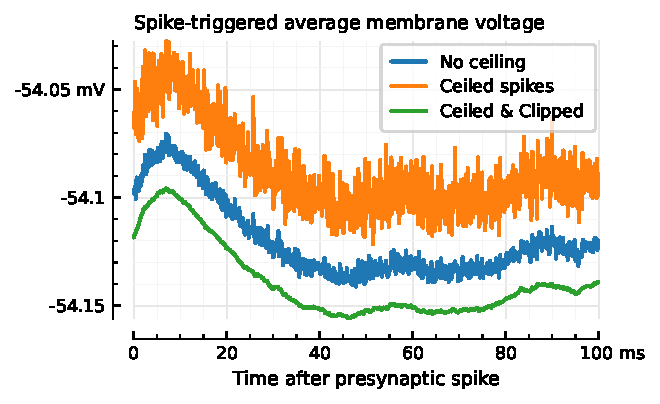
\includegraphics[w=1]{ceil_n_clip_STAs}
    \end{sidecaption}
\end{figure}

\begin{figure}
    \begin{sidecaption}
        {}
        [fig:ceil_n_clip_AUCs]
        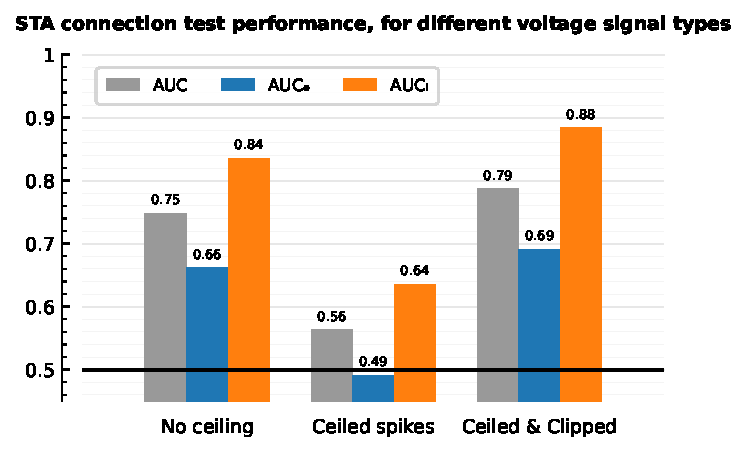
\includegraphics[w=1]{ceil_n_clip_AUCs}
    \end{sidecaption}
\end{figure}


\section{Performance quantification}

\begin{figure}
    \begin{sidecaption}
        {}
        [fig:perfmeasures_TPRs]
        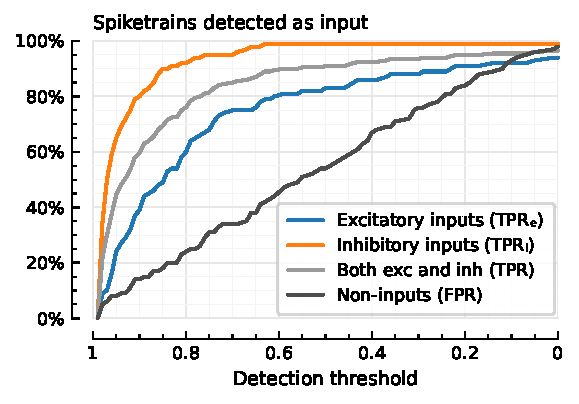
\includegraphics[w=1]{perfmeasures_TPRs}
    \end{sidecaption}
\end{figure}

\begin{figure}
    \begin{sidecaption}
        {}
        [fig:perfmeasures_ROC]
        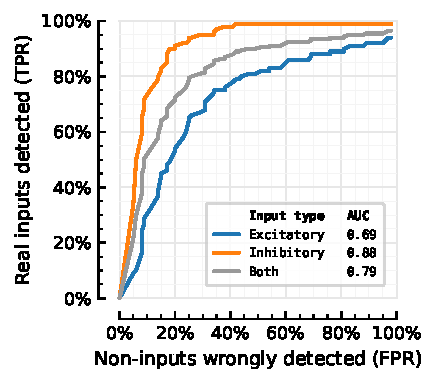
\includegraphics[w=1]{perfmeasures_ROC}
    \end{sidecaption}
\end{figure}

\begin{figure}
    \begin{sidecaption}
        {}
        [fig:perfmeasures_Fscores]
        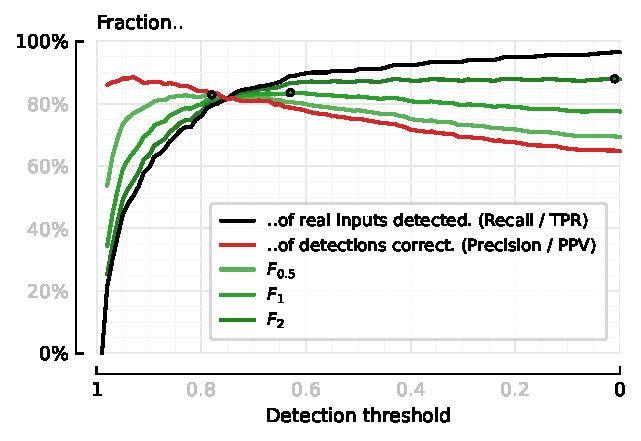
\includegraphics[w=1]{perfmeasures_Fscores}
    \end{sidecaption}
\end{figure}

\begin{figure}
    \begin{sidecaption}
        {}
        [fig:perfmeasures_PPVs]
        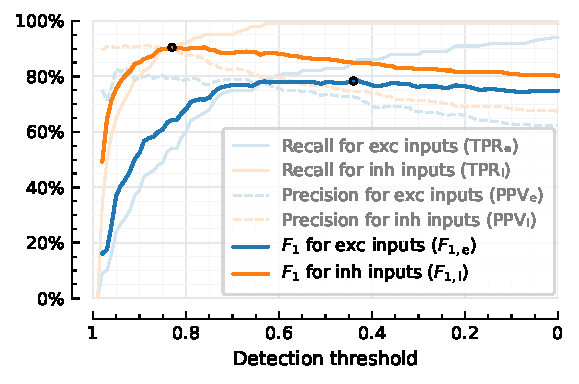
\includegraphics[w=1]{perfmeasures_PPVs}
    \end{sidecaption}
\end{figure}

\begin{figure}
    \begin{sidecaption}
        {}
        [fig:perfmeasures_PR_curves]
        \includegraphics[w=1]{perfmeasures_PR_curves_iso-Fβ}
    \end{sidecaption}
\end{figure}

\begin{figure}
    \begin{sidecaption}
        {}
        [fig:perfmeasures_PR_curves]
        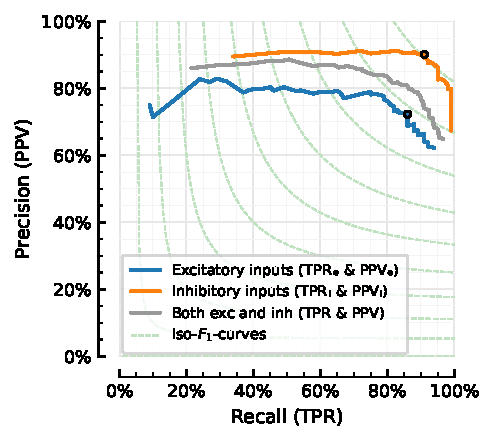
\includegraphics[w=1]{perfmeasures_PR_curves_EI}
    \end{sidecaption}
\end{figure}
